%!TEX root = ../thesis.tex

本章では, 従来研究を基にしたオフラインでデータを収集し訓練する手法を提案する.

\section{手法}

\figref{Fig:collect-data2}にデータの収集方法を示す. 赤色の線である目標経路から平行に(例:±0.10, ±0.20, ±0.30m)離れた座標にロボットを配置する. そして, その座標ごとに目標経路に沿った向きを基準として±5度傾けて, 64×48のカメラ画像(RGB画像)とルールベース制御器によるナビゲーションの出力である角速度を\figref{Fig:collect-data2}のように収集する. ロボットの進行方向に対する並進速度は0m/sであるが, データセットにはナビゲーションの出力である角速度がロボットに与えられる. \par このように, ロボットを走行させることなく, 目標経路上及び周辺に配置することで, 一度に大量のデータを収集することができる. その後, 収集したデータを用いてオフラインで学習を行う. また, 従来研究ではオンラインで学習を行うため, 計算のリソースなどの観点からバッチサイズを8にして, 全てのデータを利用してなかった(以下「従来手法」と称する). しかし, 提案手法ではオフラインで学習を行うため, バッチ学習を用いた訓練も試みる. 

% \vspace{10mm}
\newpage
  \begin{figure}[h]
  \centering
  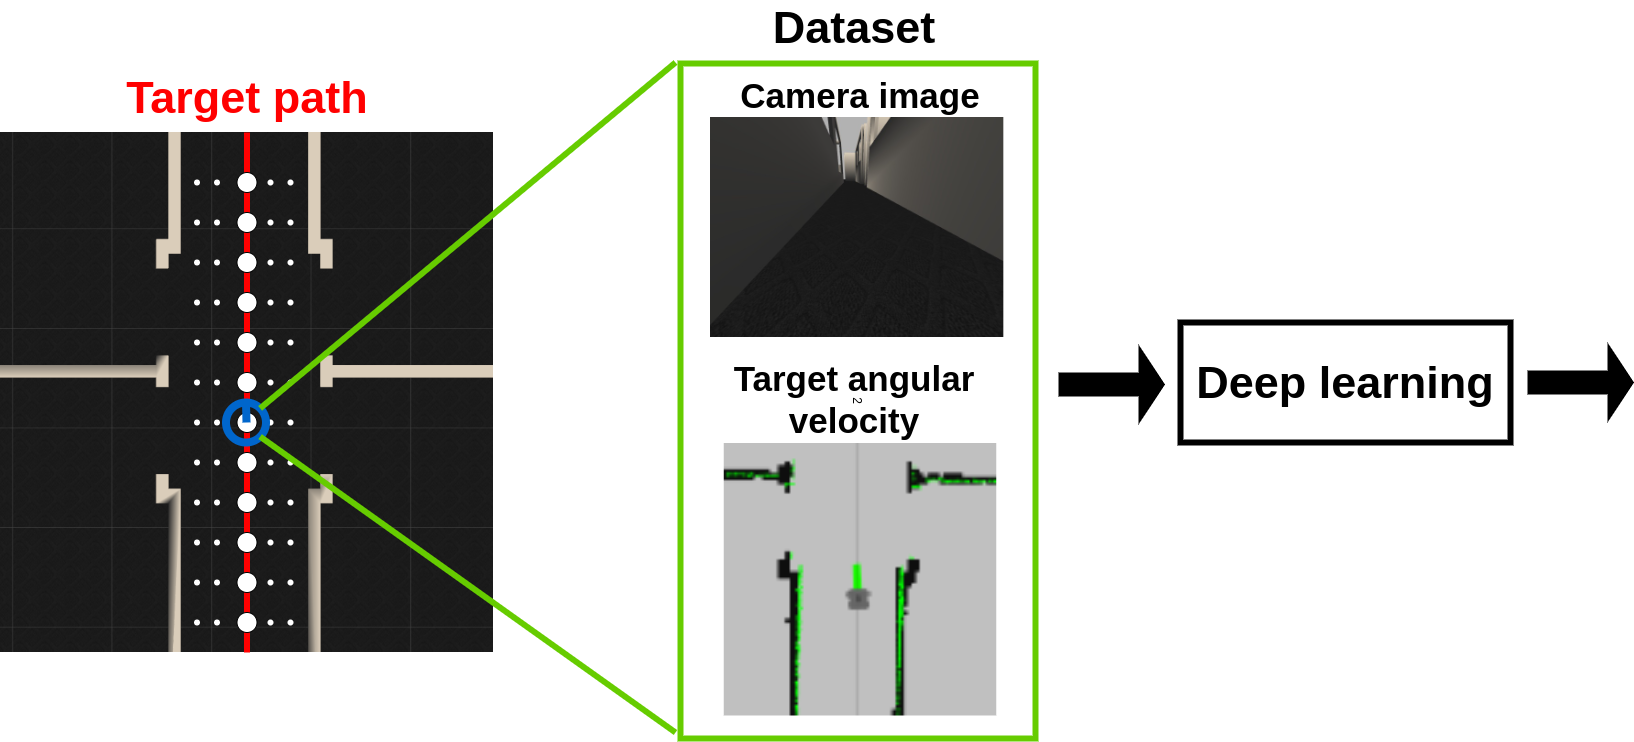
\includegraphics[keepaspectratio, scale=0.25]{images/collect-data2.png}
  \caption{Method of collecting data around the target route}
  \label{Fig:collect-data2}
  \end{figure}

